\chapter{ODE Data Representation}
In the Drasil framework, there is a single data structure containing all the information for all products; we call it \verb|System Information|. The giant \verb|System Information| collects a multitude of information; whenever we need it, we extract the information from \verb|System Information|. We store the ODE information in \verb|System Information|. 

An ODE can exist in various forms, with different forms suitable for different purposes. For example, we can transform a higher-order ODE into its equivalent system of first-order ODEs. The higher-order form is suitable for presenting the physics, but the system form is suitable for solving the ODE numerically. In previous research, we stored the ODE information in a data structure that cannot be reused for other purposes. We have to manually create the ODE in a specific form to satisfy a new goal each time. This is problematic because duplication cause problems for maintainability and traceability. In many projects, developers want to remove manually created code as much as possible because they are tedious and error-prone. For example, the \href{https://fenicsproject.org/}{FEniCS} is a project for solving differential equations. While solving differential equations with the finite element method, two variables, $A_T$ and $l_T$, are needed and usually calculated by hand (227)~\citep{loggetal2012}. To avoid creating special-purpose code, FEniCS developers decided to solve the problem by creating a form complier. Another example is the \href{https://math-atlas.sourceforge.net/}{ATLAS} project, a software tool for solving linear algebra. Researchers can implement many optimizations on specific platforms, but those optimizations may cause a slowdown on other platforms (3)~\citep{whaleyetal2001}. A traditional way of handling this problem is manually creating code for each platform. To avoid creating manually created code, ATLAS researchers decided to create a new paradigm called Automated Empirical Optimization. The Drasil team faces a similar problem: we manually extract necessary information from the original ODE. One solution is to explore a new way to store ODEs in a new data structure. The new structure must allow the different forms to be isomorphic, which means we can map one ODE form to another.

By capturing the essential information of ODEs, we can flexibly transform it into others forms that might appear. On the one hand, the transformation might result in losing information. For example, we can display an ODE in a textual form in the SRS (software requirements specification). Once we complete the transformation for displaying purposes, the textual form ODE has less information than the original ODE. On the other hand, we may make a transformation for a specific purpose, such as generating code for an ODE solver. Furthermore, capturing an ODE's information in a flexible data structure only requires a Drasil user to write the ODE's information once.

In this chapter, we will first introduce how we can rewrite ODE for a different purpose. Then, we will introduce a new data structure for storing ODE information. We will talk about details on how the new data structure captures ODE information, how to use the new data structure, and how the new data structure interacts with the Drasil Printer.

\section{Explicit Equation}
Before we conducted this project, the Drasil framework can generate software that provides numerical solutions for a first-order ODE by explicitly rewriting the ODE equation. We will rewrite the original ODE in a form which the Drasil Code Generator can utilize. The Drasil Code Generator retrieves ODE information from the new ODE form and generates a program that can produce numerical solutions. We will illustrate our steps with the \href{https://jacquescarette.github.io/Drasil/examples/nopcm/SRS/srs/NoPCM_SRS.html#Sec:IMs}{NoPCM case study}. Figure~\ref{fig_nopcm} shows how a NoPCM example works in a lab environment.
\begin{figure}[ht]
\centering
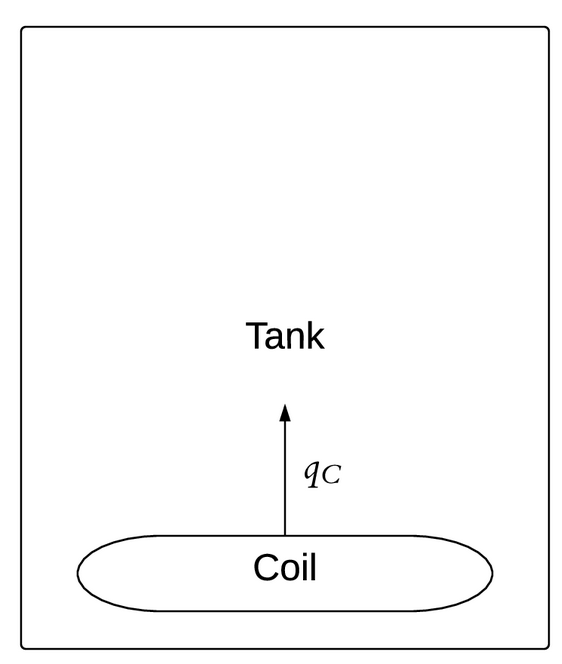
\includegraphics[width=0.3\textwidth]{figures/NoPCM.png}
\caption{NoPCM Demonstration}
\label{fig_nopcm}
\end{figure}
The rectangle represents a water tank, and it has a heating coil at the bottom of the tank. $qc$ represents the heat flux into the water from the coil. The goal is to estimate the temperature of the water over time. We can describe this natural phenomenon in a second-order ODE, Equation~\ref{eq_nopcmorginal}.

\begin{equation} \label{eq_nopcmorginal}
	T_{w}'(t) +  \frac {T_{w}(t)}{\tau_{w}} = \frac{T_{c}}{\tau_{w}}
\end{equation}
\myequations{NoPCM Equation}

$T_w(t)$ is a function of the independent variable, in this case time (t). $T_w$ is the temperature of water ($ ^\circ C $). $T_w'(t)$ is the first derivative of the function $T_w(t)$ with respect to time. $T_c$ is the temperature of the heating coil (°C), and $\tau_w$ is the ODE parameter for water related to decay time (s). Isolating for $T_w'(t)$, we obtain the following equation:
\begin{equation} \label{eq_nopcmderive}
	% T_{w}'(t) = \frac{T_{c} - T_{w}(t)}{\tau_{w}}
	T_{w}'(t) = \frac{1}{\tau_{w}} (T_{c} - T_{w}(t))
\end{equation}

\begin{listing}[ht]
\begin{haskell1}
-- Pseudocode for the readability
T_w'(t) = reciprocal τ_w * (T_c - T_w(t))
\end{haskell1}
\captionof{listing}{NoPCM Equation for SRS}
\label{code_expliciteqsrs}
\end{listing}

Based on Equation~\ref{eq_nopcmderive}, we can encode the syntax of the ODE in Code~\ref{code_expliciteqsrs} with the Drasil language. Although it has a basic mathematical structure, it is too hard-coded to make a transformation. We can use the information of Code~\ref{code_expliciteqsrs} for a display purpose, such as displaying the ODE equation in the SRS, because this form follows the syntax of the equation. However, we cannot reuse it for other purposes, such as creating a program that solves the ODE numerically. Therefore, we rewrite the Code~\ref{code_expliciteqsrs} to other forms for the purpose of solving the ODE. Brooks's thesis (91-103)~\citep{brooks} documented how the Drasil framework solves Equation~\ref{eq_nopcmderive} with the manually created \href{https://jacquescarette.github.io/Drasil/docs/drasil-code-0.1.9.0/Language-Drasil-Code.html#t:ODEInfo}{ODEInfo}. The \verb|ODEInfo| is a \verb|data type| that includes the necessary information from the original ODE (Equation~\ref{eq_nopcmderive}). The Drasil Code Generator can utilize \verb|ODEInfo| to generate a program that solves the original ODE numerically. 
\begin{listing}[ht]
\begin{haskell1}
-- Pseudocode for the readability
reciprocal τ_w * (T_c - T_w[0])
\end{haskell1}
\captionof{listing}{NoPCM Equation for the Drasil Code Generator}
\label{code_expliciteq}
\end{listing}
Code~\ref{code_expliciteq} shows how to rewrite the original ODE for the purpose of solving it. We cannot directly transform Code~\ref{code_expliciteqsrs} to Code~\ref{code_expliciteq}; there is a gap between two ODE expressions. $T\_w(t)$ is just a variable, but $T\_w[0]$ means the index of $0$ in $T\_w$. This assumes $T\_w$ is a list.

Despite the gap between Code~\ref{code_expliciteqsrs} and Code~\ref{code_expliciteq}, we can manually close it by rewriting the ODE. Rewriting the ODE in another form produces duplication because both Code~\ref{code_expliciteqsrs} and Code~\ref{code_expliciteq} describe the same ODE. The Code~\ref{code_expliciteqsrs} lacks the necessary structure to allow transformation. Therefore, we propose a new data structure to store the ODE information.

\section{Matrix Form Structure}
In general, an equation contains a left-hand expression, a right-hand expression, and an equal sign. The left-hand and right-hand expressions connect by an equal sign. A linear ODE also has its left-hand and right-hand sides. Each side has its unique shape. We can write a linear ODE in the shape of
\begin{equation} \label{eq_matrixform}
	\boldsymbol{Ax} = \boldsymbol{b}
\end{equation}
\myequations{Matrix Form}

On the left-hand side, $\boldsymbol{A}$ is an $m \times n$ matrix, and $\boldsymbol{x}$ is an $n$-vector. On the right-hand side, $\boldsymbol{b}$ is an $m$-vector. $\boldsymbol{A}$ is commonly known as the coefficient matrix, $\boldsymbol{x}$ is the unknown vector, and $\boldsymbol{b}$ is the constant vector. Equation~\ref{eq_matrixform} can represent not only a single linear ODE but also a linear system of ODEs. A linear system of ODEs is a finite set of linear differential equations. In this research, we have two case studies, NoPCM and PDController, for single higher-order linear ODEs and Double Pendulum for a system of higher-order nonlinear ODEs. The new data structure will be applied to single higher-order linear ODEs. This data structure is capable of storing information for a system of ODEs, but its related functions only support the case studies with a single ODE. Here is an ODE example from the \href{https://jacquescarette.github.io/Drasil/examples/pdcontroller/SRS/srs/PDController_SRS.html#Sec:IMs}{PDContoller case study}.
\begin{equation} \label{eq_odeexmaple}
	y''(t) + (1 + K_d) \cdot y'(t) + (20 + K_p) \cdot y(t) = r_t \cdot K_p
\end{equation}
\myequations{PDContoller Equation}

In Equation~\ref{eq_odeexmaple}, there is only one dependent variable $y$. The dependent variable $y$ is dependent on the independent variable $t$, in this case time. We use $y$(t) to represent a function of time. $y'$(t) is the first derivative of $y$(t). $y''$(t) is the second derivative of $y$(t). $y$ is the process variable, and $y'(t)$ is the rate of change of $y(t)$. $y''(t)$ is the rate of change of the rate of change of $y(t)$. $K_d$, $K_p$, and $r_t$ are constant variables. $K_d$ is Derivative Gain, $K_p$ is Proportional Gain, and $r_t$ is the Set-Point. We can write Equation~\ref{eq_odeexmaple} in a matrix form as follows:

\begin{equation} \label{eq_matrixformexmaple}
	\begin{bmatrix}
		1, & 1 + K_{d}, & 20 + K_{p}
	\end{bmatrix}
	\cdot
	\begin{bmatrix}
		y''(t)  \\
		y'(t)   \\
		y(t)  
	\end{bmatrix}
	=
	\begin{bmatrix}
		r_{t} \cdot K_{p} 
	\end{bmatrix}
\end{equation}
\myequations{PDContoller Equation in Matrix Form}

The relationship between the matrix form~\ref{eq_matrixform} and the Equation~\ref{eq_matrixformexmaple} is not hard to find. Firstly, the coefficient matrix $\boldsymbol{A}$ is a 1 $\times$ 3 matrix that consists of $1$, $1 + K_d$, ane $20 + K_p$. Secondly, the unknown vector $\boldsymbol{x}$ is a 3 $\times$ 1 vector with $y''(t)$, $y'(t)$, and $y(t)$. Lastly, the constant vector $\boldsymbol{b}$ is a 1 $\times$ 1 vector with $r_t \cdot K_p$. The matrix form~\ref{eq_matrixform} captures all the knowledge we need to present an ODE. However, what is the matrix form for a $n$th-order linear ODE? Based on Paul's Online Notes~\citep{paullinearode}, we can write all linear ODEs in the shape of

\begin{equation} \label{eq_linearDE}
	a_n(t) \cdot y^n(t) + a_{n-1}(t) \cdot y^{n-1}(t) + \dots + a_1(t) \cdot y'(t) + a_0(t) \cdot y(t) = h(t)
\end{equation}
\myequations{Linear Higher-Order ODE}

The coefficient $a_0(t), \dots, a_n(t)$ and $g(t)$ can be constant or non-constant functions, in our case they are constant functions. We also can write Equation~\ref{eq_linearDE} in a matrix form as
\begin{equation} \label{eq_matrixnthorder}
	\begin{bmatrix}
		a_n(t), & a_{n-1}, \dots, & a_0(t)
	\end{bmatrix}
	\cdot
	\begin{bmatrix}
		y^{n}(t) \\
		y^{n-1}(t) \\
		\dots \\
		y(t)  
	\end{bmatrix}
	=
	\begin{bmatrix}
		h(t)
	\end{bmatrix}
\end{equation}
\myequations{Linear Higher-Order ODE in Matrix Form}

This is the methodology used for linear ODEs, and it contains all the necessary information for understanding the linear ODE. Therefore, we create a data structure that contains the matrix information of the ODE. It is an advanced structural ODE information \verb|data type|, called \verb|DifferentialModel| to capture the knowledge of linear ODEs.

The \verb|DifferentialModel| is the type and takes one value. The \verb|SystemOfLinearODEs| is a value with a record that is used to describe the structural content of a system of linear ODEs with six necessary fields. Here is the representing code for \verb|DifferentialModel|.
\begin{haskell1}
data DifferentialModel = SystemOfLinearODEs {
	_indepVar :: UnitalChunk,
	_depVar :: ConstrConcept,
	_coefficients :: [[Expr]],
	_unknowns :: [Unknown],
	_dmConstants :: [Expr],
	_dmconc :: ConceptChunk
}
\end{haskell1}

Previous to this research, \href{https://jacquescarette.github.io/Drasil/docs/full/drasil-lang-0.1.60.0/Language-Drasil-Chunk-Unital.html#t:UnitalChunk}{UnitalChunk}, \href{https://jacquescarette.github.io/Drasil/docs/full/drasil-lang-0.1.60.0/Language-Drasil-Chunk-Constrained.html#t:ConstrConcept}{ConstrConcept}, \href{https://jacquescarette.github.io/Drasil/docs/full/drasil-lang-0.1.60.0/Language-Drasil-Expr-Lang.html#t:Expr}{Expr}, and \href{https://jacquescarette.github.io/Drasil/docs/full/drasil-lang-0.1.60.0/Language-Drasil-Chunk-Concept-Core.html#t:ConceptChunk}{ConceptChunk} already existed in Drasil. We created an \verb|Unknown| type for this experiment. Their semantics will show up in Table~\ref{tab_demodeltype}
\begin{table}[ht]
	\begin{tabular}{ p{0.2\textwidth} p{0.7\textwidth} }
		\textbf{Type} & \textbf{Semantics} \\
		\toprule
		\verb|UnitalChunk| & concepts with quantities that must have a unit definition.\\
		\verb|ConstrConcept| & conceptual symbolic quantities with Constraints and maybe a reasonable value.\\
		\verb|Expr| & a type to encode a mathematical expression. \\
		\verb|ConceptChunk| & a concept that contains an idea, a definition, and an associated domain of knowledge\\
        \verb|Unknown|& synonym of Integer\\
		\bottomrule	
	\end{tabular}	
	\caption{Type Use in DifferentialModel}	
	\label{tab_demodeltype}
\end{table}

The \verb|_indepVar| represents the independent variable, and it is often time. The \verb|_depVar| represents the dependent variable. Combing \verb|_depVar| and \verb|_indepVar|, it represents a function produce dependent variables over time. The \verb|_coefficients| is a list of lists \verb|Expr|, and it represents the coefficient matrix $\boldsymbol{A}$. The \verb|_unknowns| is a list of \verb|Unknown|, and \verb|Unknown| is a synonym of integers.
The \verb|_unknowns| represents the order of functions. Combining \verb|_depVar|, \verb|_indepVar| and \verb|_unknowns|, they can represent the unknown vector $\boldsymbol{x}$. The \verb|_dmConstants| is a list of \verb|Expr|, and it represents the constant vector $\boldsymbol{b}$. Lastly, the \verb|_dmconc| contains metadata of this model. To represent Equation~\ref{eq_odeexmaple} in \verb|DifferentialModel|, \verb|_indepVar| is time, $t$, \verb|_depVar| is $y$, \verb|_coefficients| is a 1 $\times$ 3 matrix, \verb|_unknowns| is a 3 $\times$ 1 vector, \verb|_dmConstants| is the 1 $\times$ 1 vector, and \verb|_dmconc| is \verb|ConceptChunk| that describes this model. Code~\ref{code_interaldata} shows the internal data representation of Equation~\ref{eq_odeexmaple} in \verb|DifferentialModel|.

\begin{listing}[ht]
\begin{haskell1}
_indepVar = t -- time
_depVar = y -- the dependent variable
_coefficients = [[1, 1 + K_d, 20 + K_p]]
_unknowns = [2, 1, 0] -- orders
_dmConstants = [r_t * K_p]
_dmconc = ... -- Drasil definition for chuck concept
\end{haskell1}
\captionof{listing}{Internal Data Representation for Equation~\ref{eq_odeexmaple}}
\label{code_interaldata}
\end{listing}

Currently, the \verb|DifferentialModel| only captures the knowledge of linear ODEs with one dependent variable, and it is a special case of the family of linear ODEs. Studying this special case will help the Drasil team better understand how to capture the knowledge of all ODEs and eventually lead to solving a system of linear ODE with multiple dependent variables. On top of that, there is one assumption: the \verb|_coefficients| can only be functions of independent variable \verb|_indepVar|, often time. In other words, the \verb|_coefficients| should not depend on the dependent variable \verb|_depVar|. The code does not currently check to ensure that this assumption is satisfied.

\section{Input Language}
\label{sec_input}
There are many reasons why we want to provide an input language for users to input ODE equations. One major reason is that it could be over complicated for users to input a single ODE in a matrix form. While inputting a single ODE, one obvious way is directly passing value to each record via constructors of \verb|DifferentialModel|. The Code~\ref{code_interaldata} shows how to encode Equation~\ref{eq_odeexmaple} in the \verb|DifferentialModel|. However, it would not be so elegant to set a single ODE in the example because users have to extract the coefficient matrix $\boldsymbol{A}$, unknown vector $\boldsymbol{x}$ and constant vector $\boldsymbol{b}$ from the original equation manually. Once the coefficient matrix, unknown vector and constant vector are ready, we can set values into \verb|_depVar|, \verb|_coefficients|, \verb|_unknowns|, and \verb|_dmConstants| accordingly. This process is ideal when the ODE is a system of ODE, and it would be over-complicated for a user to do extraction for a single ODE. Therefore, we decided to create a helper function to ease this issue. On top of that, the Drasil printer will print a single ODE in the SRS with a more familiar ``one line equation'' form rather than the matrix form. Another advantage of having a helper function to input an ODE is that it can reduce human error and make sure the equation is well-formed. We call this helper function the input language. We now describe this input language.

The input language is inspired by a linear $n$th-order ODE. Based on Paul's Online Notes~\citep{paullinearode}, we can write all linear ODEs in the shape of Equation~\ref{eq_linearDE}. On the left-hand side of Equation~\ref{eq_linearDE}, the expression is a collection of terms. Each term consists of a coefficient function and a derivative of the function $y(t)$. With ideas of term, coefficient, and derivative, we create new data types to mimic the mathematical expression of a linear ODE. The following is the detail of the code for new data types and operators.

\begin{haskell1}
type Unknown = Integer
data Term = T{
	_coeff :: Expr,
	_unk :: Unknown
}
type LHS = [Term]

($^^) :: ConstrConcept -> Integer -> Unknown
($^^) _ unk' = unk'

($*) :: Expr -> Unknown -> Term
($*) = T

($+) :: [Term] -> Term -> LHS
($+) xs x  = xs ++ [x]
\end{haskell1}

For the new type, \verb|LHS|, which is a short name for the left-hand side, is a list of \verb|Term|. This corresponds to the left-hand side is a collection of terms. Each \verb|Term| has an \verb|Expr| and \verb|Unknown|. This corresponds to a term consisting of a coefficient and a derivative of the function. Although \verb|_unk| is an integer, combining \verb|_unk|, \verb|_depVar| and \verb|_indepVar| we can get the derivative of the function. New operators are inspired by the linear Equation~\ref{eq_linearDE}. The \verb|$^^| operator takes a variable and an integer, and it represents the derivative of the function. For instance, in Equation~\ref{eq_odeexmaple}, we can write $y$ \$\^{}\^{} 2 to represent $y''(t)$. One thing we want to notice here is that we store $y(t)$ in \verb|_depVar| and \verb|_indepVar|. The operator \verb|$^^| will ignore the first parameter and store the second parameter in \verb|_unknowns|. The reason to position a dummy variable before \verb|$^^| is that this will maintain the whole input structure to be close to a linear ODE. The \verb|$*| operator creates a term by combining a coefficient matrix and a derivative function. For instance, in Equation~\ref{eq_odeexmaple}, we can write $(1 + K_d)\ \$*(y$ \$\^{}\^{} 1) to represent $(1 + K_d) \cdot y'(t)$. Lastly, the \verb|$+| operator will append all terms into a list. Let's write code (Code \ref{code_exinputl}) for the example matrix form~\ref{eq_odeexmaple} in the newly introduced input language. The full detail of the input language for the PDController example is shown in Appendix~\ref{const_de}.

\begin{listing}[ht]
\begin{haskell1}
-- Pseudocode for the readability
-- left hand side = y\_t'' + (1 + K\_d)y\_t' + (20 + K\_p)y\_t 
-- right hand side = r\_t K\_p

lhs = [1 $* (y $^^ 2)]
	$+ (1 + K_d) $* (y $^^ 1)
	$+ (20 + K_p) $* (y $^^ 0)
rhs = r_t * K_p
\end{haskell1}
\captionof{listing}{Input Language for Equation~\ref{eq_odeexmaple}}
\label{code_exinputl}
\end{listing}

\section{Two Constructors}
There are many ways to create the \verb|DifferentialModel|. One most obvious way is to set each field directly by passing values in the constructor, and \href{https://jacquescarette.github.io/Drasil/docs/full/drasil-lang-0.1.60.0/Language-Drasil-Chunk-DifferentialModel.html#t:makeASystemDE}{makeASystemDE} constructor serves this role. We also designed another constructor, \href{https://jacquescarette.github.io/Drasil/docs/full/drasil-lang-0.1.60.0/Language-Drasil-Chunk-DifferentialModel.html#t:makeASingleDE}{makeASingleDE}, for users who want to use the input language to create a \verb|DifferentialModel|.

For \verb|makeASystemDE| constructor, a user can set the coefficient matrix, unknown vector, and constant vector by explicitly giving \verb|[[Expr]]|, \verb|[Unknown]|, and \verb|[Expr]|. There will be several guards to check whether the inputs are well-formed, as follows:

1. The coefficient matrix and constant vector dimension need to match. The \verb|_coefficients| is an $m \times n$ matrix, and \verb|_dmConstants| is an $m$-vector. This guard makes sure they have the same $m$ dimension. If the dimensions do not match, the Drasil framework will throw an error: ``Length of coefficients matrix should be equal to the length of the constant vector''.

2. The dimension of each row in the coefficient matrix and unknown vector need to match. The \verb|_coefficients| uses a list of lists to represent an $m \times n$ matrix. It means each list in \verb|_coefficients| will have the same length $n$, and \verb|_unknowns| is an $n$-vector. Therefore, the length of each row in the \verb|_coefficients| should equal the length of \verb|_unknowns|. In the case of a size mismatch, the error message is:``The length of each row vector in coefficients needs to be equal to the length of the unknown vector''.

3. The order of the unknown vector needs to be descending due to our design decisions. We have no control over what users will give to us, and there are infinite ways to represent a linear equation in the matrix form~\ref{eq_matrixform}. We strictly ask users to input the unknown vector in descending order so that we can maintain the shape of a normal form of a linear ODE. This design decision will simplify the implementation for solving a linear ODE numerically in Chapter 3. If there is a mismatch, the error message will say, ``The order of the given unknown vector needs to be descending''.

Code~\ref{code_scexmatrix} shows how to directly set Equation~\ref{eq_odeexmaple}'s coefficient matrix, unknown vector, and constant vector. This example is made for the \href{https://jacquescarette.github.io/Drasil/examples/pdcontroller/SRS/srs/PDController_SRS.html}{PDContoller} case study.

\begin{listing}[ht]
\begin{haskell1}
-- Pseudocode for the readability
imPDRC :: DifferentialModel
imPDRC = makeASystemDE
	time
	opProcessVariable
	coeffs = [[1, 1 + K_d, 20 + K_p]]
	unknowns = [2, 1, 0]
	constants = [r_t * K_p]
	"imPDRC"
	(nounPhraseSP "Computation of the Process Variable as a function of time")
	EmptyS
\end{haskell1}
\captionof{listing}{Explicitly Set Values for Equation~\ref{eq_odeexmaple} in DifferentialModel}
\label{code_scexmatrix}
\end{listing}

The second constructor is called \verb|makeASingleDE|. This constructor uses the input language to simplify the input of a single ODE. In \verb|makeASingleDE|, we create the coefficient matrix, unknown vector, and constant vector based on restricted inputs. Contrasting to the \verb|makeASystemDE|, users have to input the ODE by using the input language we designed. In the backend, \verb|DifferentialModel| will extract useful information from the input language and generate the coefficient matrix and unknown vector. The constructor first creates a descending unknown vector base on the order of the ODE. Using Code~\ref{code_exinputl} as an example, the order of the ODE is 2, so we will generate the unknown vector $[2, 1, 0]$. Then, based on the generated unknown vector, we will search for the corresponding coefficient from the input language and form a matrix. The main advantage of this design decision is that we rely on the input language to provide the ODE in the correct format. While we allow users directly set values for \verb|DifferentialModel|, we have no guarantee the format of the input is correct. With help from the input language, users can check for syntax errors. Code~\ref{code_exinputl} shows how to use the input language to set Equation~\ref{eq_odeexmaple} in a matrix form. The full detail of how to use the input language to set the coefficient matrix, unknown vector, and constant vector for the \href{https://jacquescarette.github.io/Drasil/examples/pdcontroller/SRS/srs/PDController_SRS.html}{PDContoller} example is shown in Appendix~\ref{const_de}.

In Code~\ref{code_emulateunk}, the \verb|findHighestOrder| find the highest order $n$ in a list of \verb|Term|. Then, in \verb|createAllUnknowns|, we create a list \verb|Unknown| $[n, n-1, ..., 0]$ in descending order. This list is the \verb|_unknowns| in \verb|DifferentialModel|.

\begin{listing}[ht]
\begin{haskell1}
-- | Find the highest order in left hand side
findHighestOrder :: LHS -> Term
findHighestOrder = foldr1 (\x y -> if x ^. unk >= y ^. unk then x else y)

-- | Create all possible unknowns based on the highest order.
-- | The order of the result list is from the highest degree to zero degree.
createAllUnknowns :: Unknown -> ConstrConcept -> [Unknown]
createAllUnknowns highestUnk depv
  | highestUnk  == 0  = [highestUnk]
  | otherwise = highestUnk : createAllUnknowns (highestUnk - 1) depv
\end{haskell1}
\captionof{listing}{Emulate Unknown}
\label{code_emulateunk}
\end{listing}

Code~\ref{code_createcoe} demonstrate how to create \verb|_coefficients| for \verb|DifferentialModel|. We loop through the list of \verb|[Unknown]|. Based on each individual \verb|Unknown|, we can find its corresponding \verb|Term| in a list of \verb|Term|. We collect its \verb|Expr|. If we did not find a matched \verb|Term|, we would use 0 as the \verb|Expr|.

\begin{listing}[ht]
\begin{haskell1}
-- | Create Coefficients base on all possible unknowns
-- | The order of the result list is from the highest degree to zero degree.
createCoefficients :: LHS -> [Unknown] -> [Expr]
createCoefficients [] _ = error "Left hand side is an empty list"
createCoefficients _ [] = []
createCoefficients lhs (x:xs) = genCoefficient (findCoefficient x lhs) : createCoefficients lhs xs

-- | Get the coefficient, if it is Nothing, return zero
genCoefficient :: Maybe Term -> Expr
genCoefficient Nothing = exactDbl 0
genCoefficient (Just x) = x ^. coeff

-- | Find the term that match with the unknown
findCoefficient :: Unknown -> LHS -> Maybe Term
findCoefficient u = find(\x -> x ^. unk == u)
\end{haskell1}
\captionof{listing}{Create a Coefficient Matrix}
\label{code_createcoe}
\end{listing}

\section{Display Matrix}
After a \verb|DifferentialModel| obtains the ODE information, we want to display them in the SRS. Previously, we mentioned the Drasil framework is able to generate software artifacts, and the SRS is one of them. This section will discuss two ways to display ODEs in the SRS.

\begin{figure}[ht]
	\centering
	\begin{subfigure}[t]{\textwidth}
		\centering
		
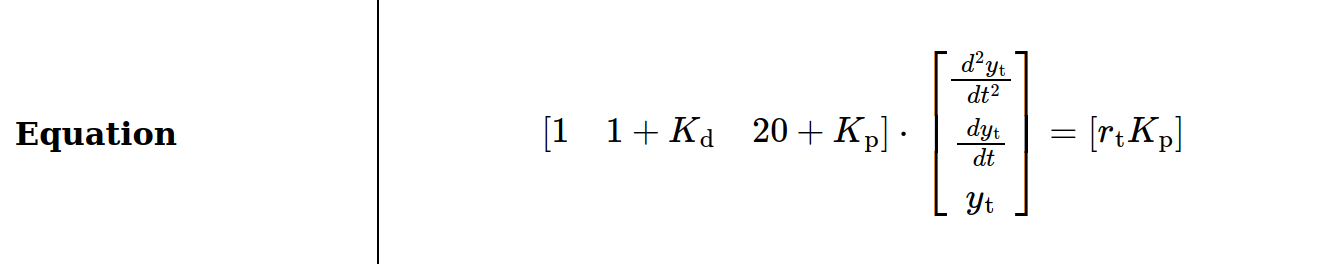
\includegraphics[width=1\textwidth]{figures/ODEInMatrix.png}
		\caption{Displaying ODE in a Matrix Form}
		\label{fig_multienv_odematrix}
	\end{subfigure}
	~
	\begin{subfigure}[t]{\textwidth}
		\centering
	
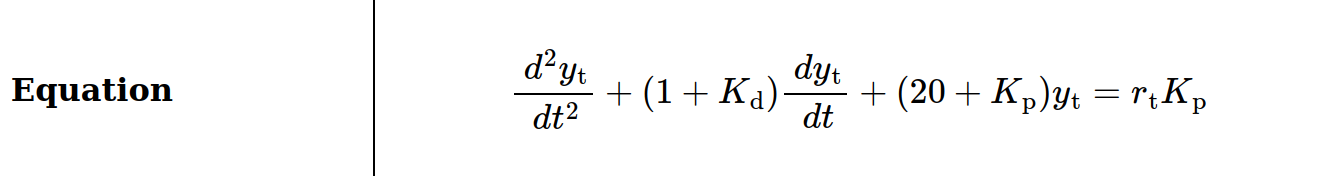
\includegraphics[width=1\textwidth]{figures/ODEInLinearEq.png}
		\caption{Displaying ODE as a Linear Equation}
		\label{fig_multienv_odelinear}
	\end{subfigure}
	
	\caption{Options of Displaying an ODE}
	\label{fig_multienv}
\end{figure}

1. We can display ODEs in a matrix form. The matrix form~\ref{eq_matrixformexmaple} is the prototype of how the ODE will appear in a matrix form in the SRS. In the \verb|DifferentialModel|, the \verb|_coefficients| is a list of lists \verb|Expr|, the unknown vector is a list of \verb|Unknown|, and the constant vector is a list of \verb|Expr|. It should be fairly straightforward for Drasil Printer to display them by printing each part sequentially. Figure~\ref{fig_multienv_odematrix} shows how to display a matrix of ODEs in the SRS. 

2. We also can display ODEs in a shape of a linear equation. Equation~\ref{eq_odeexmaple} is the prototype of how the ODE will show up in the shape of a linear equation in the SRS. Displaying a single ODE in a linear equation is a special case. When there is only one ODE, it would be over complicated to display it as a matrix. We explicitly force the Drasil printer to display a single ODE in the shape of a linear equation (Figure~\ref{fig_multienv_odelinear}). The example is just a demo that shows the Drasil printer is capable of displaying an ODE in a matrix form (Figure~\ref{fig_multienv_odematrix}).

In the future, the Drasil team wants to explore more variability in representing ODEs. An ODE has various forms, and we want \verb|DifferentialModel| to represent as many forms as possible. One topic highlighted in the discussion is showing an ODE in a canonical form. However, many mathematicians have different opinions on a canonical form, and the name of canonical form has been used differently, such as normal form or standard form. More research on this part would help us better understand the knowledge of ODE.
